\documentclass[10pt]{article}

\usepackage[margin=1in,top=0.75in]{geometry}
\usepackage{graphicx}
\usepackage{pgfgantt}
\usepackage{float}

\pagenumbering{gobble}
\setlength{\parindent}{0in}

\begin{document}
\begin{center}
	\Large\textbf{Buffalo Byte Swarm: Initial Design Memo}\\[0.1in]
	\large Group 6: Bob French, Dylan Pinos, Zhiyun Yu
\end{center}

\section*{Project Overview}
\subsection*{Problem Definition}
In disaster relief situations (earthquakes, tornadoes, etc.), rescue efforts must first search for people that require assistance before deploying a rescue team to that location. This searching stage consumes critical time in which lives could be saved, and spread resources thin as a result of having to split resources between searching and rescuing. Our project aims to eliminate this step, allowing rescue teams to begin their rescue much sooner, based on a list of suspected rescue locations.
\subsection*{Alternative Solutions}
\underline{RecoNode}: https://ieeexplore.ieee.org/abstract/document/5981569\\[0.5\baselineskip]
While our proposed Buffalo Byte mesh network offers a promising solution, alternative approaches including heterogeneous robot teams, tethered systems, WSAC networks, dual-baseband radios, vision-based AI, and real-time operating systems—can further enhance search and rescue efforts. Unlike RecoNode, which employs fully custom hardware and software, our design utilizes off-the-shelf components, making it significantly more cost-effective, scalable, and easier to deploy. Integrating insights from the RecoNode research will provide a strong technical foundation for designing a more robust disaster relief system.
\subsection*{Proposed Approach}
The approach we plan to take is to create a mesh network using a large number of Buffalo Bytes, and a central node/server, hosted on a Raspberry Pi or similar. The Buffalo Bytes will travel across the affected area and take sensor readings at certain points specified by the main node. If human presence is detected, the Buffalo Byte will send it's location through the mesh network back to the main node to signify that there may be someone in need of rescuing at that location.

\section*{Conceptual Model}
\begin{center}
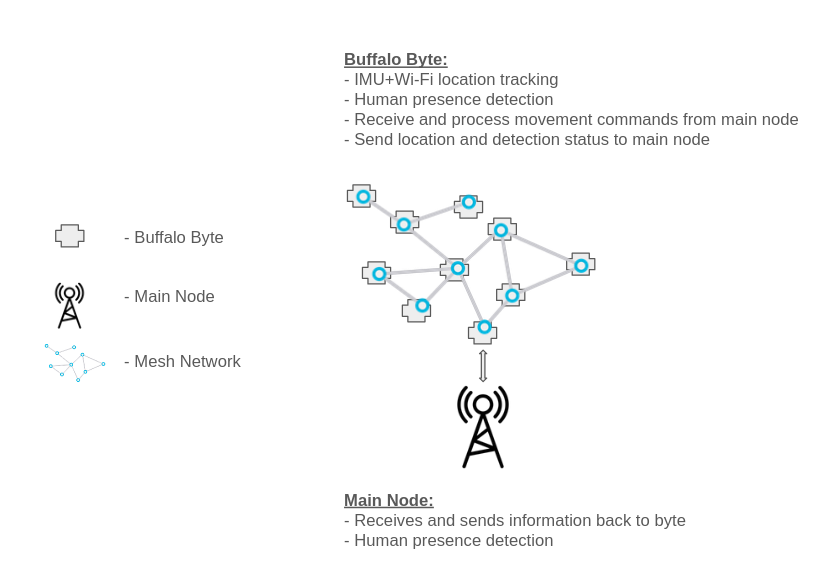
\includegraphics[scale=0.4]{conceptual-model}\\
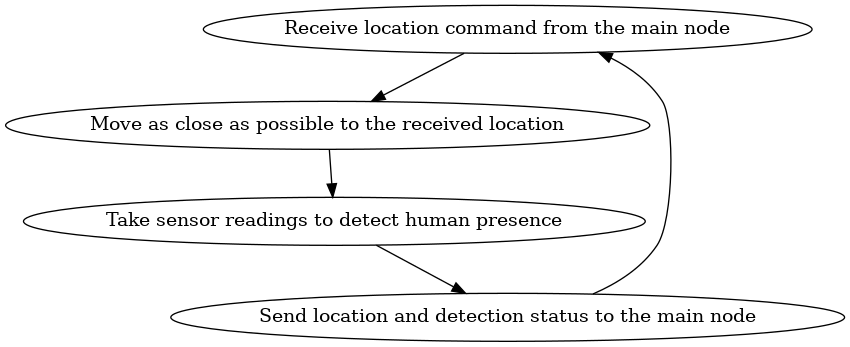
\includegraphics[scale=0.4]{state}\\
\end{center}

\section*{Measure of Success}
\subsection*{Technical Standards}
\underline{ISO 13482:2014}\\[0.25\baselineskip]
This standard describes the safety requirements for non-medical and non-industrial human aid robots, and the factors that must be satisfied in order for the robot to be considered safe for human interaction.\\[0.1in]
\underline{IEEE 42010}\\[0.25\baselineskip]
This standards describes best practice for organizing software-heavy systems in a modular manner. This will be relevant to our project because many of our subsystems are heavily software reliant. Building them in a modular way will make testing each individual components much easier as it allows for each subsystem to be tested completely isolated from the others.
\subsection*{Measurement Criteria}
\underline{Mesh Network}: Measure the average latency and packet loss when sending data over the mesh network.\\[0.5\baselineskip]
\underline{Location Tracking}: Measure the average offset between the predicted and measured location.\\[0.5\baselineskip]
\underline{Human Sensing}: Measure success rates for human detection and percentage of false positives.\\[0.5\baselineskip]
\underline{Pathfinding}: Create a list of obstacles and measure how reliably a Byte can navigate around them.
\subsection*{Measurement Plan}
When comparing possible approaches to designing a subsystem (e.g. sensor type, pathfinding algorithm, etc.), we will use the above measurement criteria to evaluate the alternatives and choose the most performant. Upon the completion of a subsystem, it will be tested by the appropriate criteria to establish a baseline measurement. As these subsystems are tweaked, we will test again to ensure that the changes result in better performance with respect to these criteria. Before implementing a design, we will check with the relevant standards mentioned above to ensure that the design would adhere to them.

\section*{Timeline}
\subsection*{Bob's Timeline}
\begin{enumerate}
	\item Create a software simulation environment for Buffalo Byte which simulates movement and IMU data
	\item Set up the mesh network, and confirm communication is possible between Bytes and the main node
	\item Create protocol for choosing a new location and sending the Byte to it
	\item Create a pathfinding algorithm for the Buffalo Byte to find the locations given to it by the main node
	\item Create the server/client applications for the Byte and the main node
	\item Conduct testing on the Byte Swarm in a physical environment, and make adjustments accordingly
\end{enumerate}
\begin{ganttchart}[bar height=0.7,y unit title=2\baselineskip,y unit chart=0.2in,vgrid,hgrid]{1}{22}
	\gantttitlelist{4,...,14}{2}\\
    \ganttbar{1}{1}{3}\\
    \ganttbar{2}{4}{6}\\
    \ganttbar{3}{7}{8}\\
    \ganttbar{4}{9}{13}\\
    \ganttbar{5}{14}{16}\\
	\ganttbar{6}{17}{20}
\end{ganttchart}
\subsection*{Dylan's Timeline}
\begin{enumerate}
	\item Write equations and create a program to track position data using the IMU and EKF
	\item Create a program to enhance this movement tracking via Wi-Fi triangulation
	\item Create a pathfinding algorithm for the Buffalo Byte to find the locations given to it by the main node
	\item Finalize and implement protocols for server/Byte communication
	\item Conduct testing on the Byte Swarm in a physical environment, and make adjustments accordingly
\end{enumerate}
\begin{ganttchart}[bar height=0.7,y unit title=2\baselineskip,y unit chart=0.2in,vgrid,hgrid]{1}{22}
	\gantttitlelist{4,...,14}{2}\\
    \ganttbar{1}{1}{5}\\
    \ganttbar{2}{6}{9}\\
    \ganttbar{3}{10}{13}\\
    \ganttbar{4}{14}{16}\\
	\ganttbar{5}{17}{20}
\end{ganttchart}
\subsection*{Zhiyun's Timeline}
\begin{enumerate}
	\item Explore sensor options and test alternatives to choose the best option
	\item Interface the selected sensor with the ESP8266
	\item Create a pathfinding algorithm for the Buffalo Byte to find the locations given to it by the main node
	\item Finalize and implement protocols for server/Byte communication
	\item Conduct testing on the Byte Swarm in a physical environment, and make adjustments accordingly
\end{enumerate}
\begin{ganttchart}[bar height=0.7,y unit title=2\baselineskip,y unit chart=0.2in,vgrid,hgrid]{1}{22}
	\gantttitlelist{4,...,14}{2}\\
    \ganttbar{1}{1}{5}\\
    \ganttbar{2}{6}{9}\\
    \ganttbar{3}{10}{13}\\
    \ganttbar{4}{14}{16}\\
	\ganttbar{5}{17}{20}
\end{ganttchart}

\end{document}
